\documentclass[12pt]{article}
\usepackage[paper=letterpaper,margin=2cm]{geometry}
\usepackage{amsmath}
\usepackage{amssymb}
\usepackage{amsfonts}
\usepackage{newtxtext, newtxmath}
\usepackage{enumitem}
\usepackage{titling}
\usepackage[colorlinks=true]{hyperref}
\usepackage[T1]{fontenc}
\usepackage{listings}
\usepackage{color}
\usepackage{graphicx}
\usepackage{tikz}
\usepackage{multicol}
\usepackage{colortbl}
\usepackage{booktabs}
\usepackage{array}
\usepackage{caption}

\definecolor{dkgreen}{rgb}{0,0.6,0}
\definecolor{gray}{rgb}{0.5,0.5,0.5}
\definecolor{mauve}{rgb}{0.58,0,0.82}

\lstset{frame=tb,
  language=Python,
  upquote=true,
  showstringspaces=false,
  columns=flexible,
  basicstyle={\small\ttfamily},
  numbers=left,
  numberstyle=\tiny\color{gray},
  keywordstyle=\color{blue},
  commentstyle=\color{dkgreen},
  stringstyle=\color{mauve},
  breaklines=true,
  breakatwhitespace=true,
  tabsize=2,
  backgroundcolor=\color{white},   % choose the background color
  captionpos=b,                    % sets the caption-position to bottom
  escapeinside={\%*}{*)},          % if you want to add LaTeX within your code
}

\begin{titlepage}
  \title{Introduction to AI}
  \author{Assignment 2}
  \date{\today}
\end{titlepage}

\begin{document}
\maketitle
\begin{enumerate}
  \usetikzlibrary{positioning, quotes}
\item For\footnote{Source code on \url{https://github.com/jinhanloh2021/AI\_AS2}} the below graph (heuristic values are provided in red color and actual costs are in black
color), please provide answers to the following answers:\\
Please note that $S$ is start and $G$ is the goal state.
\begin{center}
  \begin{tikzpicture}[
      ->,>=stealth,auto,node distance=0cm,
      thick,main node/.style={circle,draw}
    ]
    \node[main node][label={[font=\small,text=red]above:$14$}] (S) at (0,3){$S$};
    \node[main node][label={[font=\small,text=red]below:$8$}] (A) at (3,0){$A$};
    \node[main node][label={[font=\small,text=red]above right:$10$}] (B) at (3,3){$B$};
    \node[main node][label={[font=\small,text=red]above:$10$}] (C) at (3,6){$C$};
    \node[main node][label={[font=\small,text=red]below:$6$}] (D) at (6,0){$D$};
    \node[main node][label={[font=\small,text=red]above right:$4$}] (E) at (6,3){$E$};
    \node[main node][label={[font=\small,text=red]above:$6$}] (F) at (6,6){$F$};
    \node[main node][label={[font=\small,text=red]above:$1$}] (H) at (9,3)  {$H$};
    \node[main node] (G) at (12,3){$G$};

    \draw [->]
    (S)  edge["6"] (A)
    (S)  edge["4"] (B)
    (S)  edge["9"] (C)
    (A)  edge["2"] (D)
    (B)  edge["6"] (E)
    (C)  edge["4"] (F)
    (B)  edge["1"] (A)
    (B)  edge["1"] (C)
    (A)  edge["4"] (E)
    (C)  edge["4"] (E)
    (F)  edge["1"] (E)
    (D)  edge["1"] (E)
    (D)  edge["5"] (H)
    (E)  edge["3"] (H)
    (F)  edge["5"] (H)
    (H)  edge["3"] (G);
  \end{tikzpicture}
\end{center}
\begin{enumerate}
  \item Is the heuristic admissible? Provide justification. Please fill in the intermediate table below to answer this question.
        \begin{center}
          \bgroup
          \def\arraystretch{1.5}%
          \captionsetup{type=figure}
          \begin{tabular}{|c|c|c|}
            \hline
            Node $n$ & Min cost to reach $G$ from $n$ & $h(n)$ \\
            \hline
            $S$      & $14$                           & $14$   \\
            $A$      & $9$                            & $8$    \\
            $B$      & $10$                           & $10$   \\
            $C$      & $10$                           & $10$   \\
            $D$      & $7$                            & $6$    \\
            $E$      & $6$                            & $4$    \\
            $F$      & $7$                            & $6$    \\
            $H$      & $3$                            & $1$    \\
            \hline
          \end{tabular}
          \captionof{table}{Comparison of min cost to goal and heuristic for every node}
          \egroup
        \end{center}
        Since $\forall n$, $h(n)\le Mincost(n)$, the heuristic $h$ is admissible.
  \item Is the heuristic consistent? Provide justification.\\[10pt]
        A heuristic is consistent if $\forall n \ \text{and}\  \forall p$, $h(n) \le c(n,p) + h(p)$. For the given graph, the heuristic $h$ is not consistent. This can be proven by counter-example.\\
        Take node $B$ and $A$. Given
        \begin{align*}
          h(B)   & = 10 \\
          c(B,A) & = 1  \\
          h(A)   & = 8  \\
        \end{align*}
        Then
        \begin{align*}
          h(B) & > c(B,A) + h(A) \\
          10   & > 8 + 1 = 9     \\
        \end{align*}
        Hence, $h$ is not consistent.
  \item Provide the search steps (as discussed in class) with vanilla \textbf{Breadth First Search (BFS)}. Show the \textbf{final solution path} and the \textbf{cost of that solution} for each algorithm. Also compute the search steps for \textbf{A* search} with the following heuristic:\\[10pt]
        Specify for each algorithm if the open list is queue, stack or priority queue. As a simplifying assumption, let index zero (i.e first element) in the open list be the top of the stack or front of the (priority) queue, as appropriate for the corresponding algorithm. Break ties by alphabetical order.\\
        Please use the following tables for your working. Open list contains nodes that are to be explored, and "nodes to add" are the successors of the node that is recently popped or dequeued.\\[10pt]
        \textbf{Breadth First Search algorithm}
        \begin{center}
          \bgroup
          \def\arraystretch{1.5}%
          \captionsetup{type=figure}
          \begin{tabular}{|c|c|c|c|}
            \hline
            Step \# & Open Queue           & Dequeue & Nodes to add \\
            \hline
            $1$     & $S$                  & $S$     & $A,B,C$      \\
            $2$     & $A^S, B^S, C^S$      & $A$     & $D,E$        \\
            $3$     & $B^S, C^S, D^A, E^A$ & $B$     &              \\
            $4$     & $C^S, D^A, E^A$      & $C$     & $F$          \\
            $5$     & $D^A, E^A, F^C$      & $D$     & $H$          \\
            $6$     & $E^A, F^C, H^D$      & $E$     &              \\
            $7$     & $F^C, H^D$           & $F$     &              \\
            $8$     & $H^D$                & $H$     & $G$          \\
            $9$     & $G^H$                & $G$     &              \\
            \hline
          \end{tabular}
          \captionof{table}{BFS priority queue}
          \egroup
        \end{center}
        Path taken is
        $$
          S \rightarrow A \rightarrow D \rightarrow H \rightarrow G
        $$
        \begin{align*}
          cost & = 6 + 2 + 5 + 3 \\
               & = 16
        \end{align*}
        \textbf{A* Search algorithm}\\
        Let $X^n_f$ be a node $X$, where $n$ is the parent state and $f=g(X) + h(X)$ as defined by the algorithm.
        \begin{center}
          \bgroup
          \def\arraystretch{1.5}%
          \captionsetup{type=figure}
          \begin{tabular}{|c|c|c|c|}
            \hline
            Step \# & Open Priority Queue                      & Dequeue & Nodes to add \\
            \hline
            $1$     & $S$                                      & $S$     & $A,B,C$      \\
            $2$     & $A^S_{14}, B^S_{14}, C^S_{19}$           & $A$     & $D,E$        \\
            $3$     & $B^S_{14}, D^A_{14}, E^A_{14}, C^S_{19}$ & $B$     & $A,C$        \\
            $4$     & $A^B_{13}, D^A_{14}, E^A_{14}, C^B_{15}$ & $A$     & $D,E$        \\
            $5$     & $D^A_{13}, E^A_{13}, C^B_{15}$           & $D$     & $E,H$        \\
            $6$     & $E^D_{12}, H^D_{13}, C^B_{15}$           & $E$     & $H$          \\
            $7$     & $H^E_{12}, C^B_{15}$                     & $H$     & $G$          \\
            $8$     & $G^H_{14}, C^B_{15}$                     & $G$     &              \\
            \hline
          \end{tabular}
          \captionof{table}{A* search priority queue}
          \egroup
        \end{center}
        Path taken is
        $$
          S \rightarrow B \rightarrow A \rightarrow D \rightarrow E \rightarrow H \rightarrow G
        $$
        \begin{align*}
          cost & = 4 + 1 + 2 + 1 + 3 + 3 \\
               & = 14
        \end{align*}
\end{enumerate}
  \item You are hired by a moving company to move $N$ boxes from a corner of a room to the opposite
corner of the room. The room can be roughly divided into four corners, and there is an indoor
pond in the middle of the room preventing any direct diagonal crossing. The three boxes have
different sizes and can only be stacked in such a way that larger boxes can never be placed
on top of smaller ones.\\
Please answer the following questions:
\begin{enumerate}
  \item Given $N$ boxes (stacked appropriately in corner $A$ with the smallest box on the top), formulate this problem as a search problem. Indicate the
        \begin{itemize}
          \item States (describe specifically what a state is in this problem, how you would store it in a computer using a data structure, and justify the correctness of your representation)
          \item Actions
          \item Cost of different actions
          \item Successor state for each action and give one example with all of its successor states listed
          \item The objective
        \end{itemize}
        I made some assumptions for this problem:
        \begin{itemize}
          \item I can only move one box at a time
          \item I can only remove a box from the top of a stack
          \item I can only add a box to the top of a stack
          \item I cannot sort a stack in place
          \item Each room can only contain one stack
          \item All boxes have unique sizes
          \item All stacks must be appropriately placed, smallest box at top largest at bottom
        \end{itemize}
        With the rules of the game clear, we can define the state unambiguously.\\
        Let the set of rooms be $R = \{a, b, c, d\}$, a box $B$ with size $i$ be $b_i\in B=\{b_1, b_2, \ldots ,b_n\}$, a stack $G$ in room $r$ be $g(r) \subseteq B$ and a box $b_i$ in a stack $g(r)$ be $g(r,i)\in B$, the number of boxes be $N$, and the position of the mover $M$ in the room $r$ be $M = m_r$.\\
        We can then represent the start state as with $N=3$ as
        \begin{align*}
          g(a) & = \{b_1, b_2, b_3\} \\
          g(b) & = \{\emptyset\}     \\
          g(c) & = \{\emptyset\}     \\
          g(d) & = \{\emptyset\}     \\
          M    & = m_a
        \end{align*}
        And the goal state as the state where all boxes are in $g(d)$
        \begin{align*}
          g(a) & = \{\emptyset\}     \\
          g(b) & = \{\emptyset\}     \\
          g(c) & = \{\emptyset\}     \\
          g(d) & = \{b_1, b_2, b_3\} \\
          M    & = m_d
        \end{align*}
        This represents 4 stacks $g(r)$ in each room $R = \{a, b, c, d\}$, with a set of boxes. Each stack must be ordered from smallest to largest. And $M$ represents the position of the mover.\\
        To represent the state as a data structure in Python, we can use a list containing 4 stacks. Each stack represents the stack of boxes in a room. We can assign each room to each stack respectively in increasing order. The stack is implemented as an integer list and each integer represents the size of a box. The mover can be represented as a separate integer variable containing the index of the stack he is in. Here is a diagram to illustrate this model.
        \begin{center}
          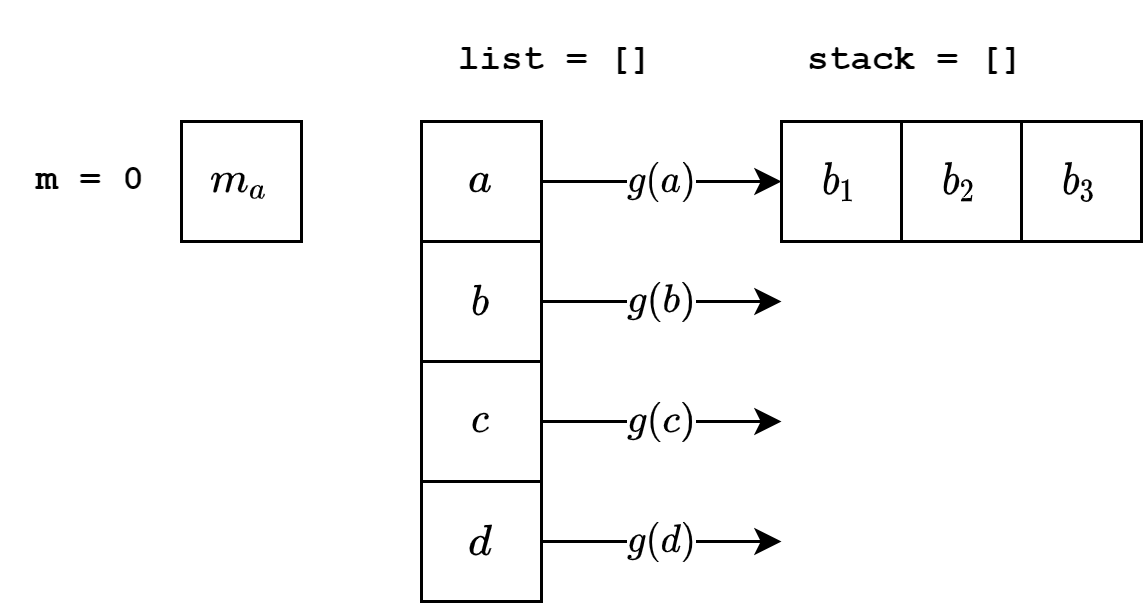
\includegraphics[scale=0.3]{"./Diagrams/Q2_DataStructure.png"}
        \end{center}
        This data structure is correct because it contains all possible positions of the boxes in every room. It also contains all possible rooms the mover can be in. It does not enforce the constraints such as the ordering or the diagonal constraint. These will be enforced by the methods we are allowed to perform on the data structure.\\
        The base action in our system is to move a box from one room to an adjacent room, subject to the system rules. This action has a cost 1. We further simplify the actions by assuming that:
        \begin{itemize}
          \item The size of the box doesn't affect the cost
          \item Moving without a box has 0 cost
          \item Appending and popping from a stack (picking up and putting down a box) costs 0
          \item Mover must be in the same room as a box to pick up or put down a box
        \end{itemize}
        For example, for an action $C(a, b), C(b, d)$ represents popping a box from the top of the stack $g(a)$ and carrying it to room $b$, then carrying it to room $d$ and appending it to the top of the stack $g(d)$. The popping and appending costs 0. The moving has a cost of $1+1=2$ as we travelled from $a\rightarrow b$ and from $b\rightarrow d$. In the implementation, there must be checks to ensure that the ordering rule is respected when appending to a stack.\\
        Here is an example of a state with $N=1$ and all successor states.
        \begin{center}
          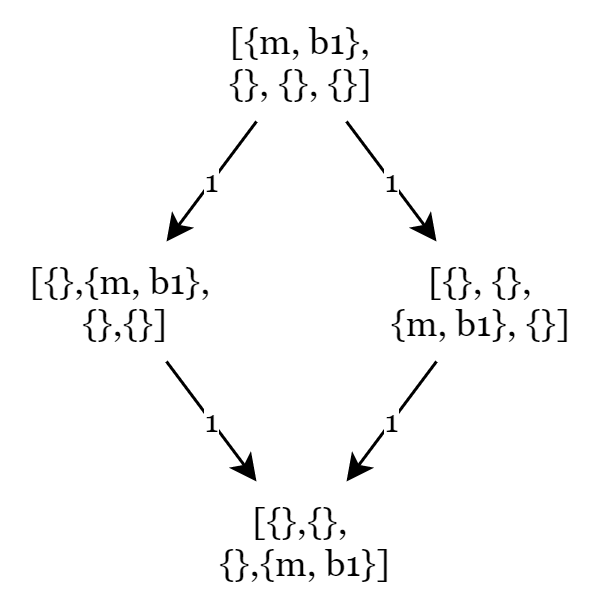
\includegraphics[scale=0.4]{"./Diagrams/Q2_StartStateWithAllSuccessorStates.png"}
        \end{center}
        This represents a start state where one box $b_1$ is in room $a$ and the mover is also in room $a$. The possible actions from the start state are to move the box to rooms $b$ or $c$, then to $d$.\\
        We can see that we have reached the goal state by completing action in two steps as all the boxes are in the room $d$.
  \item For using heuristic search methods such as A*, provide an admissible heuristic and justify why it is admissible.\\[10pt]
        An admissible heuristic for some state $n$ would be the number of boxes not in room $d$.
        $$
          h(n) = N - \lvert g(d)\rvert
        $$
        Given a base case where we have a single box in room $b$, the least cost path is 1, which is to take the box directly to $C(b,d)$. But for any other case where we have more than 1 box or if our box is located diagonally from the $d$, the cost would be greater as we cannot directly append the boxes to stack $g(d)$ as it will violate the ordering rule. We might also have to travel more than one room to reach $d$.\\
        This will always result in a cost greater than the heuristic.Thus the heuristic admissible.
  \item For the case where $N = 3$, compute the first three steps of DFS search. You can use the table structure as in question 1c to show different steps.
        \begin{center}
          \bgroup
          \def\arraystretch{1.5}%
          \captionsetup{type=figure}
          \begin{tabular}{|c|c|}
            \hline
            Step \# & Stacks                                    \\
            \hline
            $1$     & $[\{m,b_1, b_2, b_3\}, \{\}, \{\}, \{\}]$ \\
            $2$     & $[\{b_2, b_3\}, \{m,b_1\}, \{\}, \{\}]$   \\
            $3$     & $[\{m,b_2, b_3\}, \{b_1\}, \{\}, \{\}]$   \\
            \hline
          \end{tabular}
          \captionof{table}{States of stacks for first three steps of DFS}
          \egroup
        \end{center}
  \item Give a solution to the problem for $N = 3$. You can achieve it either using some methods from the class or through guessing.
        I am ignoring the position of the mover $m$ in the state here as his movement without a box costs 0. To transition from a state $[\{b_2, b_3\}, \{m,b_1\}, \{\}, \{\}]$ to $[\{m,b_2, b_3\}, \{b_1\}, \{\}, \{\}]$ costs 0, so I will omit it for brevity's sake.
        \begin{center}
          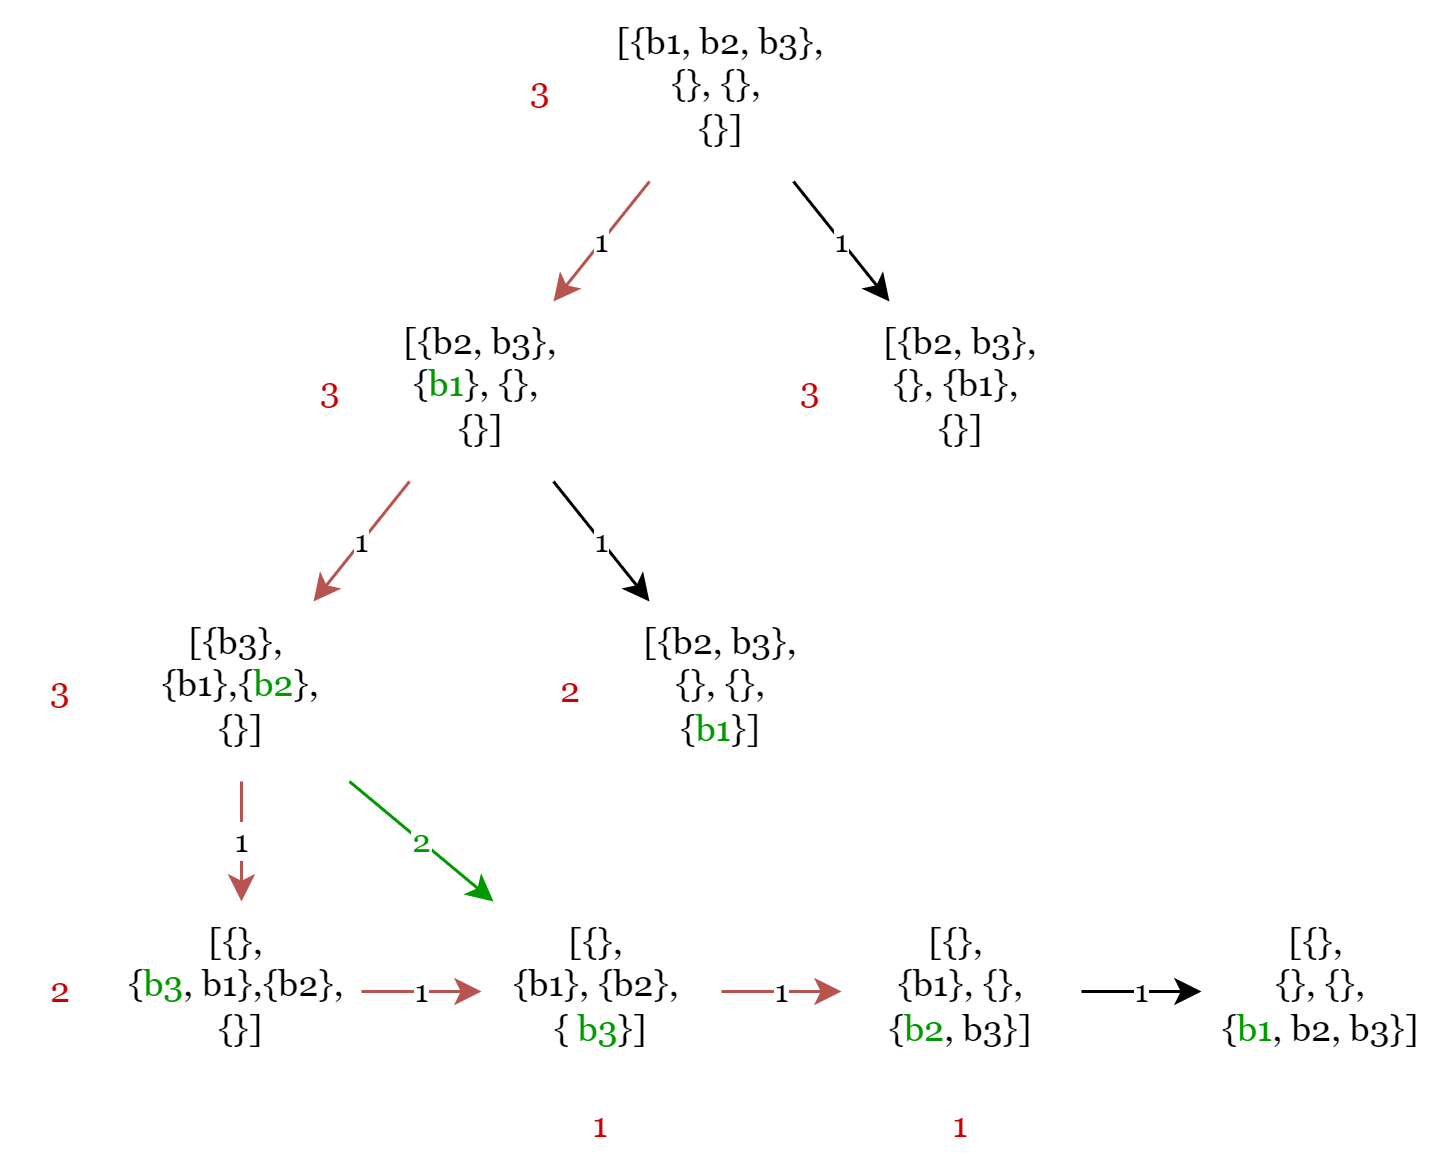
\includegraphics[scale=0.25]{"./Diagrams/DFS_Tree_Solution.png"}
        \end{center}
        The solution is shown by the red arrows. The cost of each action is shown in the arrow as black text, and the red text represents the heuristic of each state. The green elements highlights the box that is currently held by the mover. There is a green arrow which represents a "shortcut" as the mover moves from $a$ to $d$ through $c$. Note that in $[\{\}, \{b_3, b_1\}, \{b_2\}, \{\}]$ the order rule appears to be violated as $b_3$ is above $b_1$. But since the box $b_3$ is being held by the mover in room $b$, it is not violated.
  \item How would the state representation change in part A if the following modifications are applied to the problem:
        \begin{itemize}
          \item The cost to move one box is now proportional to the size of the box (cost of 1 for moving the smallest box, cost of 3 for moving the largest one).
          \item If the moving company employee moves from one corner to the other without carrying any box, it also incurs a cost of 0.5
        \end{itemize}
        For my state representation, the box representation will still work as my boxes are labelled as $b_i$ where $i$ is the weight. Similarly, the position of the mover is still the same with the new rule that movement from one corner to another without a box will cost 0.5.\\[10pt]
        The changes can be seen in the \textbf{actions} rather than in the state. Now we can redefine an action to $C(a,b,b_i)$, where the mover moves a box $b_i$ from room $a$ to $b$. Previously the cost was $1$ for any $b_i$ but the new cost will be $i$.\\
        Another change we have to make is to represent the position of the mover. Previously I ignored his position in our state representation as his movement cost without a box was 0. But now, we can have a new action $C(a,b,b_0)$ which costs 0.5, when a mover moves from room $a$ to room $b$ without a box. Now we cannot ignore the position of the mover, and we require an additional variable in our state $m$ to represent the room the mover is currently in.
\end{enumerate}
  \item Please recall the robot runner in the grid world example with tiger and food cells on right last column. The states are grid cells, i.e., $(1,1), (1,2), \ldots$. First component of a state is the row number, second component is the column number. The actions available are North, East, West, South. Rewards are given as follows:
\begin{itemize}
  \item $R(*,*,*)=-0.1$ (Penalty of movement, assuming result state is not food or tiger)
  \item $R(*,*,(3,4))=+2$ (Moving to food cell)
  \item $R(*,*,(2,4))=-1$ (Moving to tiger cell)
\end{itemize}
Transition probability is $0.5$ to the state in the direction of the action and $0.25$ in states perpendicular to the direction of the action. If agent hits a wall, the agent moves back to its original location. Terminating states are when agent is in the food cell or in the tiger cell. Discount factor is $0.95$.\\
For value iteration method, the values of different states $V^t$(.) at an iteration \textbf{t} are given by:
\begin{center}
  \bgroup
  \def\arraystretch{1.5}%
  \begin{tabular}{|c|c|c|c|c|}
    \hline
    $3$ & $0.653$ & $1.059$              & $1.381$ & Food    \\
    $2$ & $0.400$ & \cellcolor[gray]{.1} & $0.434$ & Tiger   \\
    $1$ & $0.082$ & $-0.11$              & $-0.00$ & $-0.35$ \\
    \hline
        & $1$     & $2$                  & $3$     & $4$     \\
    \hline
  \end{tabular}
  \egroup
\end{center}
\begin{enumerate}
  \item Compute the values of $V^{t+1}$(.) for different states at iteration $t+1$. The $V^{t+1}$ values for some states are given in the table below. You need to compute the values for states with "?" entry. Write numerical answers for such cells in the table below.
        \begin{center}
          \bgroup
          \def\arraystretch{1.5}%
          \begin{tabular}{|c|c|c|c|c|}
            \hline
            $3$ & $0.653$ & $1.059$              & $1.381$ & Food  \\
            $2$ & $0.400$ & \cellcolor[gray]{.1} & $0.434$ & Tiger \\
            $1$ & $0.082$ & $?$                  & $?$     & $?$   \\
            \hline
                & $1$     & $2$                  & $3$     & $4$   \\
            \hline
          \end{tabular}
          \egroup
        \end{center}
        Please show analytical expressions denoting all computations without using any python code.\\[10pt]
        For state $S=(1,3)$,
        \begin{align*}
          Q^{t+1}((1,3), N) & =\sum_{s'}P(s'\vert (1,3), N)[R((1,3), N, s') + \gamma V^t(s')]    \\
                            & =.5(-.1 + .95(.434)) + .25(-.1 + .95(-.11)) + .25(-.1 + .95(-.35)) \\
                            & = -0.00435                                                         \\
          Q^{t+1}((1,3), W) & =\sum_{s'}P(s'\vert (1,3), W)[R((1,3), W, s') + \gamma V^t(s')]    \\
                            & =.5(-.1 + .95(-.11)) + .25(-.1 + .95(.434)) + .25(-.1 + .95(0))    \\
                            & = -0.0875                                                          \\
        \end{align*}
        Taking action $S$ and $E$ are trivial, as $S$ is worse than $N$ because the successful action is greater for $N$ than $S$ and the unsuccessful action are the same. By the same logic, action $W$ is worse than $E$. Hence,
        $$
          V^{t+1}(1,3)= -0.00435
        $$
        For state $S=(1,4)$,
        \begin{align*}
          Q^{t+1}((1,4), W) & =\sum_{s'}P(s'\vert (1,4), W)[R((1,4), W, s') + \gamma V^t(s')] \\
                            & =.5(-.1 + .95(0)) + .25(-1) + .25(-.1 + .95(-.35))              \\
                            & = -0.4275                                                       \\
          Q^{t+1}((1,4), S) & =\sum_{s'}P(s'\vert (1,4), S)[R((1,4), S, s') + \gamma V^t(s')] \\
                            & =.5(-.1 + .95(-.35)) + .25(-.1 + .95(0)) + .25(-.1 + .95(-.35)) \\
                            & = -0.2075                                                       \\
        \end{align*}
        Taking action $N$ and $E$ are trivial, as $N$ is the worst move as it goes to the Tiger. Since going $W$ is worst than $S$, we can also conclude that $E$ is worse than $S$ as $E$ has a chance of meeting the Tiger which automatically decreases our utility by $0.25$. Hence,
        $$
          V^{t+1}(1,4)= -0.2075
        $$
        For state $S=(1,2)$,
        \begin{align*}
          Q^{t+1}((1,2), W) & =\sum_{s'}P(s'\vert (1,2), W)[R((1,2), W, s') + \gamma V^t(s')]     \\
                            & =.5(-.1 + .95(0.082)) + .25(-.1 + .95(-.11)) + .25(-.1 + .95(-.11)) \\
                            & = -0.1236                                                           \\
        \end{align*}
        Taking action $W$ is the only action with a positive successful state. The other actions have negative successful states.
        $$
          V^{t+1}(1,2)= -0.1236
        $$
        Hence, at $V^{t+1}$
        \begin{center}

          \bgroup
          \def\arraystretch{1.5}%
          \begin{tabular}{|c|c|c|c|c|}
            \hline
            $3$ &     &                      &            & Food      \\
            $2$ &     & \cellcolor[gray]{.1} &            & Tiger     \\
            $1$ &     & $-0.1236$            & $-0.00435$ & $-0.2075$ \\
            \hline
                & $1$ & $2$                  & $3$        & $4$       \\
            \hline
          \end{tabular}
          \egroup
        \end{center}
        \clearpage
  \item What is the policy for each state as per the function $Q^{t+1}$(..). Note it down below for each entry with "?" mark.
        \begin{center}
          \bgroup
          \def\arraystretch{1.5}%
          \begin{tabular}{|c|c|c|c|c|}
            \hline
            $3$ & $E$ & $E$                  & $E$ & Food  \\
            $2$ & $N$ & \cellcolor[gray]{.1} & $N$ & Tiger \\
            $1$ & $N$ & $W$                  & $N$ & $S$   \\
            \hline
                & $1$ & $2$                  & $3$ & $4$   \\
            \hline
          \end{tabular}
          
          \egroup
        \end{center}
        From the $Q^{t+1}$ I've calculated in the previous part, the optimal policy is shown in the diagram above.
\end{enumerate}
  \item In this question, you will employ Singular Value Decomposition to obtain word embeddings and compare the generated word embeddings with the word embeddings generated using word2vec. The corpus to be considered is a set of tweets posted about the Covid- 19 pandemic on Twitter (\lstinline{Corona_Tweets.csv}), which is a real-life dataset. You need to do the following (code template provided is \lstinline{Q4_template_tweets.ipynb} you are free to use helper functions if required):\\
\begin{enumerate}
  \item Update the \lstinline{load_data} function from the \lstinline{Q4_template_tweets.ipynb} to preprocess words: remove non-letters, convert words into the lower case, and remove the stop words. You can employ some functions from the \lstinline{NLP-pipeline-example.ipynb} example and may use regular expressions from \lstinline{Word2Vec.ipynb}. {\bf [2 marks]}
        \begin{lstlisting}
    def load_data():
      """ Read tweets from the file.
          Return:
              list of lists (list_words), with words from each of the processed tweets
      """
      tweets = pd.read_csv('/content/drive/MyDrive/Colab Notebooks/AI_AS2/Corona_Tweets.csv', names=['text'])
      list_words = []
      ### iterate over all tweets from the dataset
      for i in tweets.index:
        ### remove URLs
        text = re.sub("https?://\S+|www\.\S+", " ", tweets.loc[i, 'text'])
        ### remove non-letter.
        text = re.sub("[^a-zA-Z]"," ",text)
        ### tokenize
        words = text.split()
        
        new_words = []
        ### iterate over all words of a tweet
        for w in words:
          ## TODO: remove the stop words and convert a word (w) to the lower case
          stops = set(stopwords.words("english"))
          if w not in stops:
            new_words.append(w.lower())
          
        list_words.append(new_words)
      return list_words
  \end{lstlisting}
  \item Create the co-occurrence matrix for all the remaining words (after stop words are eliminated), where the window of co-occurrence is 5 on either side of the word. What is the size of your vocabulary (i.e., how many unique words you end up with)? \textbf{[4 marks]}
        \begin{lstlisting}
    def distinct_words(corpus):
      """ get a list of distinct words for the corpus.
          Params:
              corpus (list of list of strings): corpus of documents
          Return:
              corpus_words (list of strings): list of distinct words across the corpus, sorted (using python 'sorted' function)
              num_corpus_words (integer): number of distinct words across the corpus
      """
      corpus_words = set()
      for tweet in corpus:
        for word in tweet:
          corpus_words.add(word)
      corpus_words = sorted(list(corpus_words))
      num_corpus_words = len(corpus_words)
      return corpus_words, num_corpus_words

    words, num_words = distinct_words(twitter_corpus) # 11454 unique words
  \end{lstlisting}
        \begin{lstlisting}
    def compute_co_occurrence_matrix(corpus, window_size=5):
      """ Compute co-occurrence matrix for the given corpus and window_size (default of 5).
          Params:
              corpus (list of list of strings): corpus of documents
              window_size (int): size of context window
          Return:
              M (numpy matrix of shape = [number of corpus words x number of corpus words]): 
                  Co-occurence matrix of word counts. 
                  The ordering of the words in the rows/columns should be the same as the ordering of the words given by the distinct_words function.
              word2Ind (dict): dictionary that maps word to index (i.e. row/column number) for matrix M.
      """
      M = np.zeros((num_words, num_words), dtype=int)
      word2Ind = {}
      for i, w in enumerate(words):
        word2Ind[w] = i
      for tweet in corpus:
        for i, w in enumerate(tweet):
          w_idx = word2Ind[w]
          start = i - 5
          end = i + 5 + 1 #exclusive
          for j in range(start, end):
            if(i != j and j >= 0 and j < len(tweet)):
              c_idx = word2Ind[tweet[j]]
              M[w_idx, c_idx] += 1
              M[c_idx, w_idx] += 1
      return M, word2Ind

    M, word2Ind = compute_co_occurrence_matrix(twitter_corpus)
  \end{lstlisting}
        The number of unique vocabulary is $11454$.
  \item Apply SVD and obtain word embeddings of size 75. {\bf [2 marks]}
        \begin{lstlisting}
    # -----------------------------
    # Run SVD
    # Note: This may take several minutes (~20-30 minutes)
    # ------------------------------
    la = np.linalg
    U, s, Vh = la.svd(M, full_matrices=False)

    # Compute SVD embeddings
    embedding_size = 75
    SVD_embeddings = np.dot(U[:,:embedding_size], np.diag(s[:embedding_size]))
  \end{lstlisting}
  \item Then, please generate word embeddings of size 75 using \lstinline{Word2Vec.ipynb} (uploaded in class lecture material) on the same dataset. Please show comparison on few examples to understand which method works better. You may use the \lstinline{svd.most_similar} function from the template to perform the comparisons. Note your observations in your solution. You can use words like “covid”, “grocery” etc to compare the two models. {\bf [2 marks]}
        \begin{lstlisting}
    # Creating the word2vec model and setting values for the various parameters
    # Initializing the train model. 
    num_features = 75   # Word vector dimensionality
    min_word_count = 0  # Minimum word count. You can change it also.
    num_workers = 4     # Number of parallel threads, can be changed
    context = 5         # Context window size
    downsampling = 1e-3 # (0.001) Downsample setting for frequent words, can be changed
    # Initializing the train model
    print("Training Word2Vec model....")
    model = word2vec.Word2Vec(twitter_corpus,
                              workers=num_workers,
                              vector_size=num_features, # API Change to vector_size
                              min_count=min_word_count,
                              window=context,
                              sample=downsampling)

    # To make the model memory efficient
    model.init_sims(replace=True)
  \end{lstlisting}
        \begin{lstlisting}
    def svd_most_similar(query_word, n=10):
        """ return 'n' most similar words of a query word using the SVD word embeddings similar to word2vec's most_similar    
            Params:
                query_word (strings): a query word
            Return:
                most_similar (list of strings): the list of 'n' most similar words
        """
        # get index of a query_word
        query_word_idx = word2Ind[query_word]
        # get word embedding for a query_word
        word = SVD_embeddings[query_word_idx]
        #cosine similarity matrix
        cos_similarity = cosine_similarity(SVD_embeddings, word.reshape(1, -1))
        most_similar = []
        # model.wv.most_similar(query_word)
        '''
            Write additional code to compute the list most_similar. Each entry in the list is a tuple (w, cos)
            where w is one of the most similar word to query_word and cos is cosine similarity of w with query_word
        '''
        # get index of top n most similar words
        similar_i = np.argsort(-cos_similarity.flatten())[1:n+1]
        
        # get similar words and cos_sim score
        for i in similar_i:
          word = list(word2Ind.keys())[i]
          cos_sim = cos_similarity[i][0]
          most_similar.append((word, cos_sim))

        # sort decreasing based on second item in tuple
        most_similar.sort(key=lambda x: x[1], reverse=True)

        return most_similar
  \end{lstlisting}
        \begin{lstlisting}
    svd_most_similar("covid")
    model.wv.most_similar("covid") #this word2vec trained model on tweets
    svd_most_similar("grocery")
    model.wv.most_similar("grocery")
  \end{lstlisting}
        \begin{center}
          \bgroup
          \def\arraystretch{1.5}%
          \captionsetup{type=figure}
          \begin{tabular}{|c|c c|c c|}
            \hline
            {}   & \multicolumn{2}{c|}{\textbf{covid}} & \multicolumn{2}{c|}{\textbf{grocery}}                            \\
            \hline
            Rank & SVD                                 & word2vec                              & SVD           & word2vec \\
            \hline
            {1}  & outbreak                            & panicbuying                           & mailing       & went     \\
            {2}  & pandemic                            & coronaoutbreak                        & mall          & shelves  \\
            {3}  & new                                 & coronavirus                           & liquor        & empty    \\
            {4}  & check                               & pandemic                              & ht            & local    \\
            {5}  & fear                                & coronavirusoutbreak                   & accusations   & today    \\
            {6}  & due                                 & lockdown                              & elys          & no       \\
            {7}  & toiletpaper                         & corona                                & llama         & retail   \\
            {8}  & change                              & coronapocalypse                       & dollargeneral & bread    \\
            {9}  & probably                            & uk                                    & pajama        & packs    \\
            {10} & news                                & due                                   & quarterly     & pasta    \\
            \hline
          \end{tabular}
          \captionof{table}{Similar words for covid and grocery for each model}
          \egroup
        \end{center}
\end{enumerate}
  \item In this question, you need to install OpenAI gym:
\begin{itemize}
  \item \href{https://github.com/openai/gym}{\color{blue}Installation Instructions}
  \item \href{https://www.gymlibrary.dev/content/basic_usage/}{\color{blue}Documentation}
\end{itemize}
Once the gym is installed, you have to implement Q-learning for the \href{https://www.gymlibrary.dev/environments/toy_text/frozen_lake/}{\color{blue}\lstinline{FrozenLake-v1}
  environment} in python using the gym library and show the rewards obtained. Use option \lstinline{is_slippery=True}. Use map size 4x4 (check option '\lstinline{map_name}').\\
You may use a discount factor $\gamma = 0.95$. Please provide the following things in your solution for this question:
\begin{enumerate}
  \item Code that implements Q-learning for the \lstinline{FrozenLake-v1} example in the gym? Copy and paste the code in the solution pdf, and provide the actual code file also. A key thing to determine first is what is the size of the state space and action space in this environment to make the appropriate data structures such as the Q-table \textbf{[6 points]}
  \item For each episode, compute the total accumulated reward (also called episode return). Plot the average return (over the last 50 episodes) while your agent is learning (x-axis will be the episode number, y-axis will be the average return over the last 50 episodes). Make sure that you train for sufficiently many episodes so that convergence occurs. \textbf{[3 points]}
  \item What is the epsilon you used for epsilon-greedy exploration and how did you select this epsilon $\varepsilon$? What would happen if you use a high epsilon such as $\varepsilon = 0.5$? \textbf{[1 point]}
\end{enumerate}
\end{enumerate}

\end{document}
